% --------------------------------------------------------------------------
% Artigo sobre o Método Simplex - Formatado para IEEE Conference Template
% Este documento é auto-contido e usa o Noto Sans como fonte principal.
% --------------------------------------------------------------------------
\documentclass[conference]{IEEEtran}

% --- Pacotes Essenciais ---
\usepackage{amsmath}     % Para equações matemáticas avançadas
\usepackage{booktabs}    % Para tabelas com qualidade de publicação (\toprule, \midrule, \bottomrule)
\usepackage{xcolor}      % Para definir cores, usado no realce de código
\usepackage{listings}    % Para formatar blocos de código (Python)
\usepackage{url}         % Para formatar URLs corretamente (especialmente na bibliografia)
\usepackage{cite}        % Para formatar citações no estilo IEEE (ex: [1]-[3])
\usepackage{graphicx}
% --- Configuração de Idioma e Fonte (Protocolo Padrão) ---
% Usa babel para hifenização e termos em português
\usepackage[portuguese, provide=*]{babel}
\babelprovide[import, onchar=ids fonts]{portuguese}
\babelprovide[import, onchar=ids fonts]{english}
\usepackage{fontspec}    % Permite o uso de fontes OpenType (como Noto)
\babelfont{rm}{Noto Sans} % Define Noto Sans como a fonte principal
\babelfont[portuguese]{rm}{Noto Sans} % Garante que o português use a fonte

% Correção para listas em idiomas não-ingleses
\usepackage{enumitem}
\setlist[itemize]{label=-}

% --- Configuração do Pacote Listings para Python ---
\definecolor{codegray}{rgb}{0.5,0.5,0.5}
\definecolor{codepurple}{rgb}{0.58,0,0.82}
\definecolor{backcolour}{rgb}{0.95,0.95,0.95}

\lstdefinestyle{pythonstyle}{
    backgroundcolor=\color{backcolour},   
    commentstyle=\color{codegray},
    keywordstyle=\color{blue},
    stringstyle=\color{codepurple},
    basicstyle=\ttfamily\footnotesize,
    breakatwhitespace=false,         
    breaklines=true,                 
    captionpos=b,                    
    keepspaces=true,                 
    numbers=left,                    
    numbersep=5pt,                  
    showspaces=false,                
    showstringspaces=false,
    showtabs=false,                  
    tabsize=2,
    language=Python
}
\lstset{style=pythonstyle} % Define o estilo 'pythonstyle' como padrão

% --- Hyperref (Deve ser o último pacote) ---
\usepackage{hyperref}
\hypersetup{
    colorlinks=true,
    linkcolor=blue,
    filecolor=magenta,      
    urlcolor=cyan,
    pdftitle={O Método Simplex: Otimização Prática com Python},
    pdfauthor={}
}

% --- Correção de Conflito (Babel e IEEEtran) ---
% Redefine \markboth para ser compatível com as mudanças do babel
\makeatletter
\def\markboth#1#2{\def\leftmark{\@IEEEcompsoconly{\sffamily}\MakeUppercase{#1}}%
\def\rightmark{\@IEEEcompsoconly{\sffamily}\MakeUppercase{#2}}}
\makeatother

% --------------------------------------------------------------------------
% --- Metadados do Documento ---
% --------------------------------------------------------------------------
\title{O Método Simplex:\\ Otimização Prática com Python}

% Bloco de autor como placeholder
\author{
      \IEEEauthorblockN{Sarpa, Mauricio}
    \IEEEauthorblockA{\textit{Engenharia da Computação} \\
    \textit{Fundação Hermínio Ometto}\\
    Araras, Brasil\\
    sarpa@alunos.fho.edu.br}
    \and

    \IEEEauthorblockN{Da Cunha, Julio Cezar}
    \IEEEauthorblockA{\textit{Engenharia da Computação} \\
    \textit{Fundação Hermínio Ometto}\\
    Araras, Brasil\\
    Juliocezar@alunos.fho.edu.br}
    \and

    \IEEEauthorblockN{Buzatto, Diogo}
    \IEEEauthorblockA{\textit{Engenharia da Computação} \\
    \textit{Fundação Hermínio Ometto}\\
    Araras, Brasil\\
    diogobuzatto@alunos.fho.edu.br}
    \and

    \IEEEauthorblockN{Silva, Lucas Ferreira}
    \IEEEauthorblockA{\textit{Engenharia da Computação} \\
    \textit{Fundação Hermínio Ometto}\\
    Araras, Brasil\\
    lucas.silva2958@alunos.fho.edu.br}
    \and
}

% --------------------------------------------------------------------------
% --- Início do Documento ---
% --------------------------------------------------------------------------
\begin{document}

% Cria o título
\maketitle

% --- Resumo (Abstract) ---
\begin{abstract}
Este artigo apresenta um relatório exaustivo sobre o método Simplex, um algoritmo fundamental para a resolução de problemas de Programação Linear (PL). Partindo de uma introdução aos conceitos de otimização, o texto explora os fundamentos matemáticos que sustentam o algoritmo, incluindo sua interpretação geométrica e a formulação matricial. A metodologia do Simplex tabular é detalhada passo a passo, servindo como base para uma implementação  em Python. Um estudo de caso prático sobre otimização de transporte é modelado e resolvido, com visualização dos resultados.
\end{abstract}

% --- Palavras-Chave ---
\begin{IEEEkeywords}
Método Simplex, Programação Linear, Otimização, Python, Pesquisa Operacional.
\end{IEEEkeywords}

% --------------------------------------------------------------------------
% --- Corpo do Artigo ---
% --------------------------------------------------------------------------

\section{Introdução \\ à Programação Linear e ao Método Simplex}

\subsection{O Desafio da Otimização no Mundo Moderno}
A otimização é um pilar central na tomada de decisões estratégicas em um mundo caracterizado pela abundância de dados e pela escassez de recursos. Em sua essência, otimizar significa encontrar a melhor solução possível para um problema, dadas certas limitações ou condições. A modelagem matemática surge como uma ferramenta indispensável nesse contexto, permitindo que problemas complexos do mundo real sejam representados de forma simplificada e estruturada por meio de uma linguagem universal: a matemática \cite{andrade}. Essa abordagem possibilita a análise de diferentes cenários de forma mais rápida e econômica do que a experimentação prática, oferecendo um suporte robusto ao processo decisório em áreas tão diversas quanto logística, finanças, produção industrial e engenharia \cite{andrade}.

\subsection{Programação Linear: Uma Ferramenta para a Tomada de Decisão}
Dentro do vasto campo da otimização matemática, a Programação Linear (PL) destaca-se como uma das técnicas mais importantes e bem estudadas \cite{lima}. Um problema de PL consiste em encontrar o valor máximo ou mínimo de uma função linear, denominada \textbf{função objetivo}, que está sujeita a um conjunto de restrições lineares na forma de igualdades ou desigualdades \cite{lima}. É crucial entender que o termo "programação" neste contexto não se refere à programação de computadores, mas sim ao planejamento e à alocação ótima de recursos.

Os componentes fundamentais de um modelo de Programação Linear são:
\begin{itemize}
    \item \textbf{Função Objetivo:} Uma expressão matemática linear que define a quantidade a ser otimizada. Por exemplo, em um contexto empresarial, pode ser a maximização do lucro ou a minimização dos custos de produção \cite{menezes}. Matematicamente, é expressa como $Z = c_1x_1 + c_2x_2 + \dots + c_nx_n$.
    \item \textbf{Variáveis de Decisão:} São as incógnitas do problema, representadas por $x_1, x_2, \dots, x_n$. Elas quantificam as decisões a serem tomadas, como a quantidade de cada produto a ser fabricado ou o montante a ser investido em diferentes ativos \cite{menezes}.
    \item \textbf{Restrições:} São um conjunto de equações ou inequações lineares que representam as limitações do sistema, como disponibilidade de matéria-prima, capacidade de armazenamento, horas de mão de obra ou demanda de mercado \cite{menezes}.
\end{itemize}

\subsection{O Surgimento e a Importância do Método Simplex}
Para solucionar problemas de PL com mais de duas ou três variáveis de decisão, onde métodos gráficos se tornam impraticáveis, é necessário um algoritmo mais robusto \cite{barboza}. O \textbf{método Simplex}, desenvolvido por George Dantzig em 1947, foi um marco na história da programação matemática e simboliza o início da era moderna da otimização \cite{cordeiro}. Considerado um dos algoritmos mais importantes do século XX, o Simplex é um procedimento numérico, iterativo e matricial projetado para encontrar sistematicamente a solução ótima de um modelo de PL \cite{macambira}.

A relevância do método Simplex transcende a teoria acadêmica, sendo uma ferramenta ativamente empregada para gerar valor econômico e eficiência na indústria brasileira. Uma análise da produção científica nacional revela uma forte conexão entre a teoria da Pesquisa Operacional e a prática da engenharia \cite{silva2018}. Estudos de caso demonstram sua aplicação bem-sucedida em diversos setores: na maximização do uso de matéria-prima em uma fábrica de semicondutores na Zona Franca de Manaus, resultando em uma redução de 92\% no desperdício \cite{pereira}; na otimização do mix de produção (embora em panificação, o princípio é similar ao de laticínios) \cite{milhomem}; e na melhoria de processos em microempresas do setor têxtil \cite{silva2018}. Essa ponte entre a academia e a indústria evidencia que a maestria do método Simplex e sua implementação computacional em linguagens como Python é uma habilidade de alto valor e aplicabilidade direta no mercado brasileiro.

\section{Fundamentos Matemáticos do Algoritmo Simplex}
A eficácia do método Simplex está ancorada em uma base matemática sólida que conecta conceitos de álgebra linear e geometria. Para que o algoritmo possa ser aplicado, o problema de PL deve ser primeiramente convertido para um formato padronizado.

\subsection{A Forma Padrão (FP)}
O método Simplex opera sobre problemas de PL que estão na chamada \textbf{Forma Padrão} (ou Forma Canônica). Esta forma possui características específicas que facilitam o início do procedimento algorítmico \cite{macambira}. Um problema de PL está na Forma Padrão se satisfaz as seguintes condições:
\begin{enumerate}
    \item É um problema de \textbf{maximização}.
    \item Todas as restrições são equações de igualdade (com exceção das restrições de não negatividade).
    \item O lado direito de cada restrição (termo independente $b_i$) é não negativo ($b_i \ge 0$).
    \item Todas as variáveis de decisão são não negativas ($x_j \ge 0$).
\end{enumerate}

Qualquer problema de PL pode ser convertido para a Forma Padrão através das seguintes transformações:
\begin{itemize}
    \item Um problema de minimização de uma função $Z$ é equivalente à maximização de $-Z$ \cite{milhomem}.
    \item Uma restrição de desigualdade do tipo $\sum a_{ij}x_j \le b_i$ é convertida em uma igualdade pela adição de uma \textbf{variável de folga}.
    \item Uma restrição de desigualdade do tipo $\sum a_{ij}x_j \ge b_i$ é convertida em uma igualdade pela subtração de uma \textbf{variável de excesso}.
    \item Uma variável de decisão $x_j$ que é "livre em sinal" pode ser substituída pela diferença de duas novas variáveis não negativas: $x_j = x_j' - x_j''$, onde $x_j' \ge 0$ e $x_j'' \ge 0$.
\end{itemize}

\subsection{Variáveis de Folga e Excesso}
As \textbf{variáveis de folga} são um conceito central na preparação de um problema para o Simplex. Elas são adicionadas a restrições do tipo "menor ou igual a" ($\le$) para transformá-las em igualdades. Fisicamente, uma variável de folga representa a quantidade de um recurso que não foi utilizada \cite{silva2017}. Por exemplo, a restrição $2x_1 + 3x_2 \le 100$ (horas de máquina) é convertida para $2x_1 + 3x_2 + s_1 = 100$, onde $s_1 \ge 0$ é a variável de folga que representa o número de horas de máquina ociosas \cite{menezes}.

De forma análoga, as \textbf{variáveis de excesso} são subtraídas de restrições do tipo "maior ou igual a" ($\ge$) para convertê-las em igualdades. Elas representam a quantidade pela qual o lado esquerdo da inequação excede o lado direito. A restrição $x_1 + x_2 \ge 50$ (demanda mínima) torna-se $x_1 + x_2 - e_1 = 50$, onde $e_1 \ge 0$ é a variável de excesso.


\section{O Método Simplex Tabular: Um Guia Passo a Passo}
O método Simplex tabular, é uma representação matricial que organiza os coeficientes do problema de PL e facilita a aplicação mecânica das iterações do algoritmo. Ele é uma forma concisa de acompanhar as trocas de variáveis e a evolução da solução \cite{menezes}.

\subsection{Construção do Tableau Inicial}
Para um problema de maximização na Forma Padrão, o tableau inicial é construído da seguinte forma:
\begin{enumerate}
    \item A função objetivo, por exemplo $Z = c_1x_1 + c_2x_2$, é reescrita como $Z - c_1x_1 - c_2x_2 = 0$.
    \item Cria-se uma tabela. As colunas correspondem a cada variável de decisão ($x_i$), cada variável de folga ($s_j$) e ao lado direito das equações (RHS).
    \item As linhas correspondem a cada restrição. A última linha (linha Z) representa a função objetivo.
    \item Os coeficientes das restrições são preenchidos nas linhas correspondentes.
    \item Na linha Z, inserem-se os coeficientes da função objetivo reescrita ($-c_i$). O valor inicial de Z (geralmente 0) é colocado na coluna RHS da linha Z.
\end{enumerate}
A solução básica inicial geralmente consiste nas variáveis de folga, que formam uma matriz identidade dentro do tableau \cite{menezes}.

\subsection{O Processo Iterativo}
O algoritmo Simplex é um processo iterativo que se repete até que a solução ótima seja encontrada. Cada iteração consiste nos seguintes passos:

\textbf{Passo 1: Verificação da Condição de Otimalidade}
A solução atual é ótima se todos os coeficientes na linha Z forem não negativos (para maximização) \cite{menezes}. Se sim, o algoritmo termina.

\textbf{Passo 2: Escolha da Variável de Entrada (Coluna Pivô)}
Se a condição não for atendida, a variável associada ao coeficiente mais negativo (menor valor) na linha Z é escolhida para entrar na base. Esta é a \textbf{coluna pivô} \cite{menezes}.

\textbf{Passo 3: Escolha da Variável de Saída (Linha Pivô)}
Realiza-se o \textbf{teste da razão mínima}. Para cada linha das restrições, divide-se o valor da coluna RHS pelo coeficiente correspondente na coluna pivô (apenas denominadores positivos). A linha com a menor razão não negativa é a \textbf{linha pivô} \cite{menezes}.

\textbf{Passo 4: Operação de Pivoteamento}
O elemento na interseção da coluna pivô e linha pivô é o \textbf{elemento pivô}. O objetivo é transformar a coluna pivô em uma coluna da matriz identidade usando operações elementares de linha (eliminação de Gauss-Jordan) \cite{menezes}.

\textbf{Passo 5: Repetição}
Após o pivoteamento, o processo retorna ao Passo 1.

A Tabela \ref{tab:simplex_iter} demonstra este processo para o problema: Maximizar $Z = 3x_1 + 5x_2$ sujeito a $x_1 \le 4$, $2x_2 \le 12$ e $3x_1 + 2x_2 \le 18$.

% Tabela 1 - Iterações do Simplex
\begin{table}[h]
\caption{Resolução de Exemplo pelo Método Simplex Tabular}
\label{tab:simplex_iter}
\centering
\fontsize{8}{10}\selectfont
\setlength{\tabcolsep}{4pt} % Reduz o espaço entre colunas

\textbf{Tableau Inicial (Iteração 0)}
\begin{tabular}{cccccccc}
\toprule
Base & $x_1$ & $x_2$ & $s_1$ & $s_2$ & $s_3$ & RHS & Razão \\
\midrule
$s_1$ & 1 & 0 & 1 & 0 & 0 & 4 & - \\
$s_2$ & 0 & \textbf{2} & 0 & 1 & 0 & 12 & $12/2 = 6$ \\
$s_3$ & 3 & 2 & 0 & 0 & 1 & 18 & $18/2 = 9$ \\
\midrule
Z & -3 & \textbf{-5} & 0 & 0 & 0 & 0 & \\
\bottomrule
\end{tabular}

\vspace{0.3cm}
\textbf{Tableau Após Iteração 1}
\begin{tabular}{cccccccc}
\toprule
Base & $x_1$ & $x_2$ & $s_1$ & $s_2$ & $s_3$ & RHS & Razão \\
\midrule
$s_1$ & 1 & 0 & 1 & 0 & 0 & 4 & $4/1 = 4$ \\
$x_2$ & 0 & 1 & 0 & 0.5 & 0 & 6 & - \\
$s_3$ & \textbf{3} & 0 & 0 & -1 & 1 & 6 & $6/3 = 2$ \\
\midrule
Z & \textbf{-3} & 0 & 0 & 2.5 & 0 & 30 & \\
\bottomrule
\end{tabular}

\vspace{0.3cm}
\textbf{Tableau Após Iteração 2 (Ótimo)}
\begin{tabular}{cccccccc}
\toprule
Base & $x_1$ & $x_2$ & $s_1$ & $s_2$ & $s_3$ & RHS & Razão \\
\midrule
$s_1$ & 0 & 0 & 1 & 1/3 & -1/3 & 2 & \\
$x_2$ & 0 & 1 & 0 & 1/2 & 0 & 6 & \\
$x_1$ & 1 & 0 & 0 & -1/3 & 1/3 & 2 & \\
\midrule
Z & 0 & 0 & 0 & 1.5 & 1 & 36 & \\
\bottomrule
\end{tabular}
\end{table}

\subsection{Interpretando a Solução Final}
No tableau final (Tabela \ref{tab:simplex_iter}):
\begin{itemize}
    \item As variáveis básicas são $s_1=2$, $x_2=6$, $x_1=2$.
    \item As variáveis não básicas são $s_2=0$, $s_3=0$ \cite{menezes}.
    \item A solução ótima é $x_1 = 2$, $x_2 = 6$.
    \item O valor máximo é $Z = 36$ \cite{menezes, silva2017}.
\end{itemize}

\subsection{Casos Especiais: O Método das Duas Fases}
Quando restrições do tipo $\ge$ ou $=$ existem, a base inicial de folga não é viável. Nesses casos, \textbf{variáveis artificiais} são adicionadas para criar uma base inicial \cite{milhomem, silva2017}. O \textbf{Método das Duas Fases} é aplicado:

\begin{itemize}
    \item \textbf{Fase I:} Minimiza-se a soma das variáveis artificiais. Se o mínimo for zero, uma SBV para o problema original foi encontrada, e passa-se para a Fase II. Se o mínimo for maior que zero, o problema original é inviável \cite{schneider, silva2017}.
    \item \textbf{Fase II:} O tableau final da Fase I (sem as variáveis artificiais) é usado como ponto de partida. O Simplex padrão é aplicado à função objetivo original \cite{schneider}.
\end{itemize}


\section{Otimização Linear com  Python }
Para aplicações práticas, é mais eficiente usar bibliotecas que separam a \textbf{modelagem} da \textbf{resolução}. O usuário descreve o problema, e a biblioteca invoca um \textbf{solver} de alto desempenho.

\subsection{Por que Usar Bibliotecas? }
Bibliotecas como `SciPy` e `PuLP` são interfaces para solvers poderosos (CBC, GLPK, Gurobi, CPLEX), que são motores computacionais otimizados em C++ ou Fortran, capazes de resolver problemas de larga escala com rapidez e estabilidade numérica \cite{cordeiro}.


\subsection{SciPy.optimize.linprog: Otimização Baseada em Matrizes}
A função `linprog` do SciPy é a ferramenta padrão no ecossistema científico do Python. Ela requer que o problema seja fornecido em formato matricial.

É fundamental notar que `linprog`, por padrão, resolve problemas de \textbf{minimização}. Para maximizar $Z$, deve-se minimizar $-Z$, passando o vetor `c` com sinais trocados.

\begin{lstlisting}
from scipy.optimize import linprog
import numpy as np

# Maximizar Z = 3x1 + 5x2  =>  Minimizar -Z = -3x1 - 5x2
c_scipy = np.array([-3, -5])

# Restrições (todas já são <=)
A_ub_scipy = np.array([[1, 0], [0, 2], [3, 2]])
b_ub_scipy = np.array([4, 12, 18])

# Limites (x1 >= 0, x2 >= 0)
x1_bounds = (0, None)
x2_bounds = (0, None)

# Resolver o problema (method='highs' é o padrão atual)
resultado = linprog(c_scipy, A_ub=A_ub_scipy, 
                    b_ub=b_ub_scipy, 
                    bounds=[x1_bounds, x2_bounds], 
                    method='highs')

if resultado.success:
    print("--- Solução Ótima (SciPy) ---")
    # O valor da função é negativo
    print(f"Valor Z máximo: {-resultado.fun:.2f}") 
    print(f"x1 = {resultado.x[0]:.2f}")
    print(f"x2 = {resultado.x[1]:.2f}")
else:
    print(f"Solução não encontrada: {resultado.message}")
\end{lstlisting}

\subsection{PuLP: Modelagem Algébrica Intuitiva}
PuLP permite definir problemas de PL usando uma sintaxe próxima da notação matemática, tornando o código mais legível \cite{cordeiro}.

\begin{lstlisting}
import pulp

# 1. Inicializar o modelo
modelo = pulp.LpProblem("Exemplo_Maximizacao", 
                         pulp.LpMaximize)

# 2. Definir as variáveis
x1_pulp = pulp.LpVariable('x1', lowBound=0)
x2_pulp = pulp.LpVariable('x2', lowBound=0)

# 3. Adicionar a função objetivo
modelo += 3*x1_pulp + 5*x2_pulp, "Funcao_Objetivo"

# 4. Adicionar as restrições
modelo += x1_pulp <= 4, "Restricao_1"
modelo += 2*x2_pulp <= 12, "Restricao_2"
modelo += 3*x1_pulp + 2*x2_pulp <= 18, "Restricao_3"

# Resolver o problema (usa o solver CBC por padrão)
modelo.solve()

print("--- Solução Ótima (PuLP) ---")
print(f"Status: {pulp.LpStatus[modelo.status]}")
print(f"Valor Z máximo: {pulp.value(modelo.objective):.2f}")
print(f"x1 = {pulp.value(x1_pulp):.2f}")
print(f"x2 = {pulp.value(x2_pulp):.2f}")
\end{lstlisting}

A sintaxe do PuLP é mais declarativa, sendo preferida para prototipagem rápida. 



\section{Estudo de Caso: Otimização de um Problema de Transporte}
Este estudo de caso aborda o clássico \textbf{Problema de Transporte}, que busca determinar o plano de distribuição de menor custo de origens para destinos, respeitando ofertas e demandas. 

\subsection{Formulação do Problema}
Considere 2 fábricas e 3 centros de distribuição.

\begin{itemize}
    \item \textbf{Oferta (Capacidade):}
    \begin{itemize}
        \item Fábrica 1 (BH): 1000 unidades
        \item Fábrica 2 (CP): 1500 unidades
    \end{itemize}
    \item \textbf{Demanda (Necessidade):}
    \begin{itemize}
        \item CD 1 (RJ): 800 unidades
        \item CD 2 (SP): 900 unidades
        \item CD 3 (CT): 600 unidades
    \end{itemize}
\end{itemize}

\textbf{Custos de Transporte (R\$/unidade):}
\begin{table}[h]
\centering
\begin{tabular}{lccc}
\toprule
\textbf{De / Para} & \textbf{CD 1 (RJ)} & \textbf{CD 2 (SP)} & \textbf{CD 3 (CT)} \\
\midrule
Fábrica 1 (BH) & 5 & 4 & 7 \\
Fábrica 2 (CP) & 6 & 3 & 5 \\
\bottomrule
\end{tabular}
\end{table}

\textbf{Modelagem Matemática:}

Seja $x_{ij}$ a quantidade transportada da fábrica $i$ para o CD $j$.

\textbf{Função Objetivo (Minimizar Custo Total):}
\begin{equation}
\min Z = 5x_{11} + 4x_{12} + 7x_{13} + 6x_{21} + 3x_{22} + 5x_{23}
\end{equation}

\textbf{Restrições de Oferta ($\le$):}
\begin{gather}
x_{11} + x_{12} + x_{13} \le 1000 \quad (\text{Fábrica 1}) \\
x_{21} + x_{22} + x_{23} \le 1500 \quad (\text{Fábrica 2})
\end{gather}

\textbf{Restrições de Demanda ($\ge$):}
\begin{gather}
x_{11} + x_{21} \ge 800 \quad (\text{CD 1}) \\
x_{12} + x_{22} \ge 900 \quad (\text{CD 2}) \\
x_{13} + x_{23} \ge 600 \quad (\text{CD 3})
\end{gather}

\textbf{Não Negatividade:} $x_{ij} \ge 0$.

\subsection{Resolução com Python e Análise dos Resultados}
A estrutura matricial do problema é ideal para `scipy.optimize.linprog`.

\begin{lstlisting}
import numpy as np
from scipy.optimize import linprog

# Coeficientes da função objetivo (c)
# Ordem: x11, x12, x13, x21, x22, x23
c_transporte = np.array([5, 4, 7, 6, 3, 5])

# Restrições de desigualdade (A_ub @ x <= b_ub)
# Convertendo demanda (>=) para (<=) multiplicando por -1
A_transporte = np.array([
    # Oferta (<=)
    [1, 1, 1, 0, 0, 0],   # Fábrica 1
    [0, 0, 0, 1, 1, 1],   # Fábrica 2
    # Demanda (convertida de >= para <=)
    [-1, 0, 0, -1, 0, 0],  # Demanda CD 1
    [0, -1, 0, 0, -1, 0],  # Demanda CD 2
    [0, 0, -1, 0, 0, -1]   # Demanda CD 3
])

b_transporte = np.array([
    1000, # Oferta F1
    1500, # Oferta F2
    -800, # Demanda CD 1
    -900, # Demanda CD 2
    -600  # Demanda CD 3
])

# Limites (todas as variáveis >= 0)
bounds = [(0, None) for _ in range(len(c_transporte))]

# Resolver
resultado_transporte = linprog(c_transporte, 
                             A_ub=A_transporte, 
                             b_ub=b_transporte, 
                             bounds=bounds, 
                             method='highs')

if resultado_transporte.success:
    print("\n--- Plano de Transporte Ótimo ---")
    print(f"Custo Total Mínimo: R$ {resultado_transporte.fun:.2f}")
    solucao = resultado_transporte.x.reshape(2, 3)
    print("Plano de Distribuição (unidades):")
    print("           | CD 1 (RJ) | CD 2 (SP) | CD 3 (CT)")
    print(f"Fáb. 1 (BH) | {solucao[0, 0]:9.0f} | {solucao[0, 1]:9.0f} | {solucao[0, 2]:9.0f}")
    print(f"Fáb. 2 (CP) | {solucao[1, 0]:9.0f} | {solucao[1, 1]:9.0f} | {solucao[1, 2]:9.0f}")
\end{lstlisting}

\subsection{Visualização dos Resultados}
A comunicação eficaz dos resultados é crucial. A visualização de dados serve como ponte entre a análise complexa e a inteligência de negócios \cite{cordeiro}. O código Matplotlib para gerar o gráfico de barras foi omitido, mas a Figura \ref{fig:Figure_1} representa a saída visual esperada em Grafico de barras e na Figura \ref{fig:Figure_2} esta uma representação em grafos, mostrando como sera a distribuição de uma forma mais dinâmica e visual.

\begin{figure*}[htbp]
  \centering
  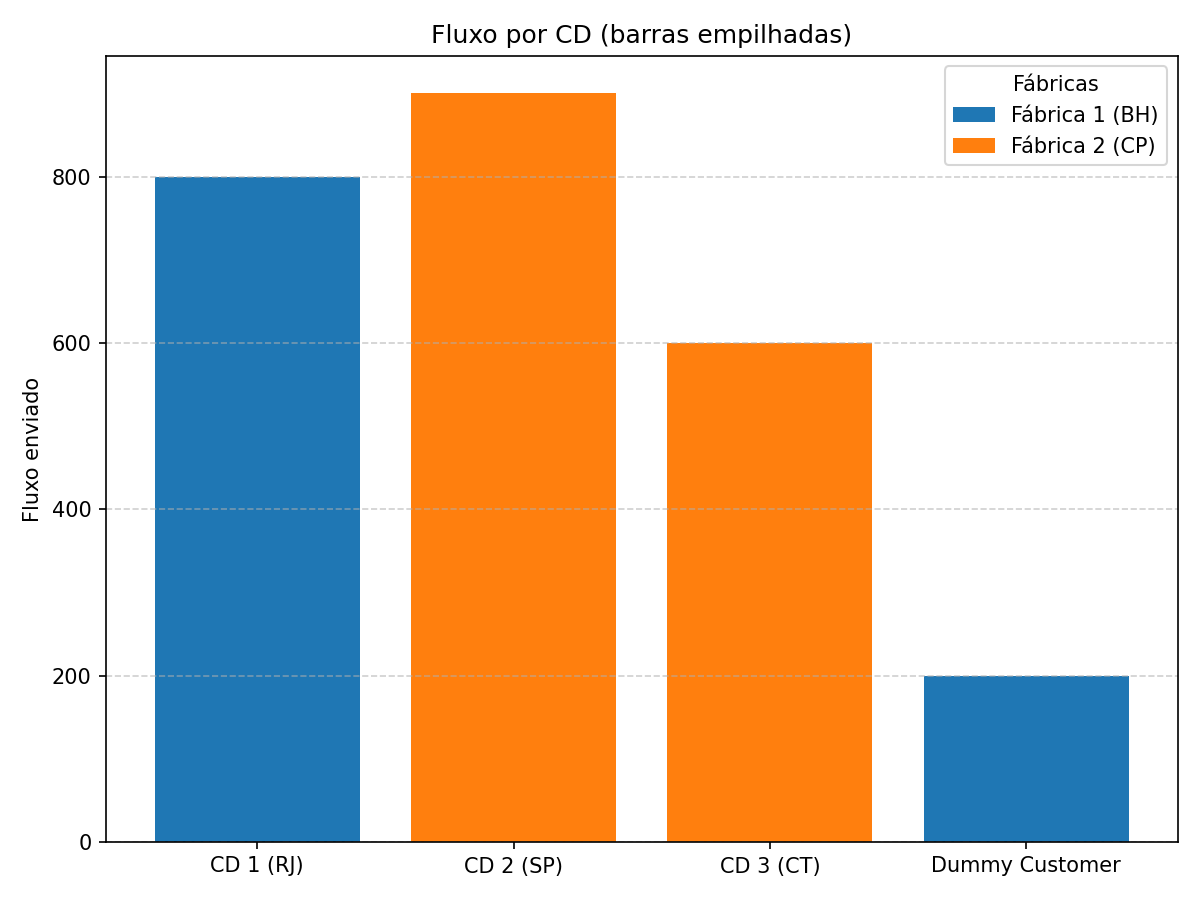
\includegraphics[width=2\columnwidth]{Figure_1.png}
  \caption{Visualização do Plano de Distribuição Ótimo (Gráfico de Barras Empilhadas). Esta figura ilustra como cada CD é abastecido pelas fábricas, conforme a solução ótima.}
  \label{fig:Figure_1} 

  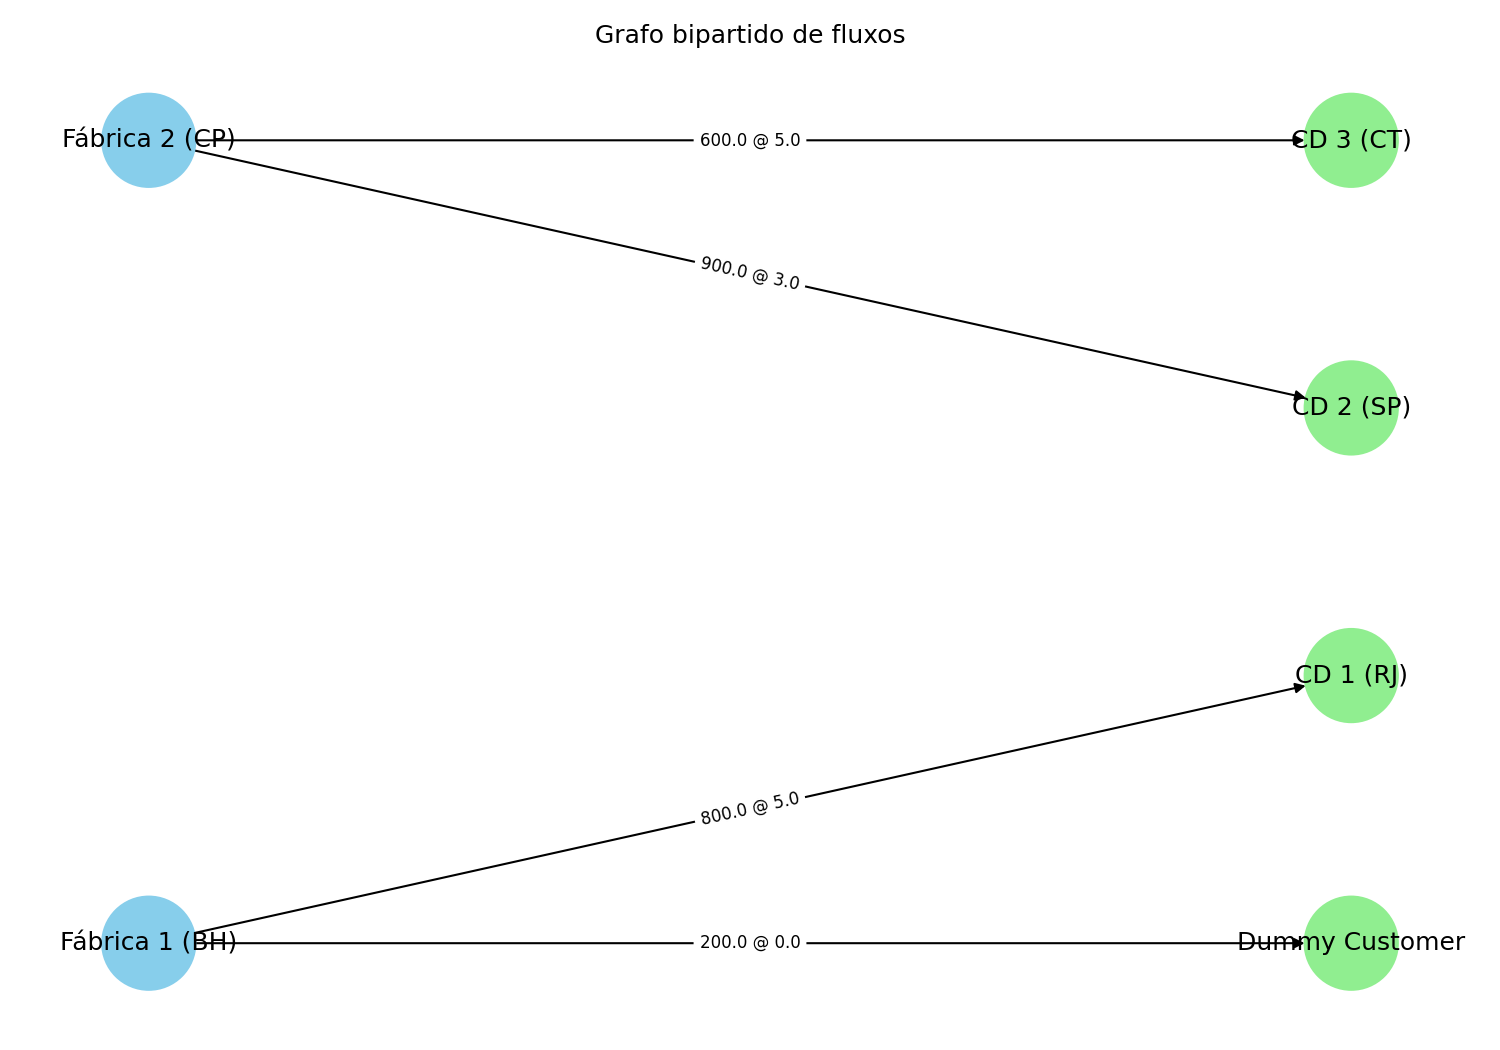
\includegraphics[width=2\columnwidth]{Figure_2.png}
  \caption{Visualização do Plano de Distribuição Ótimo (Gráfico de Barras Empilhadas). Esta figura ilustra como cada CD é abastecido pelas fábricas, conforme a solução ótima.}
  \label{fig:Figure_2} 
  
\end{figure*}


\section{Conclusão}
Este artigo percorreu o método Simplex, desde seus fundamentos teóricos até sua aplicação prática em Python. A construção de um solver "do zero" com NumPy desmistificou o algoritmo, mas também evidenciou as limitações que justificam o uso de bibliotecas profissionais como `SciPy` e `PuLP`.

Ficou claro que, para aplicações práticas, estas ferramentas são preferenciais, permitindo ao analista focar na modelagem. A sintaxe algébrica do PuLP destaca-se pela clareza. O estudo de caso do Problema de Transporte consolidou a aplicação e ressaltou a importância da visualização de dados para comunicar a solução. O método Simplex, combinado com Python, permanece uma ferramenta de otimização atemporal, impulsionando a eficiência na indústria e academia brasileira \cite{cordeiro, silva2018}.

% --------------------------------------------------------------------------
% --- Bibliografia ---
% --------------------------------------------------------------------------
% Formato IEEE (manual, usando thebibliography)
\begin{thebibliography}{99}

\bibitem{andrade}
E. L. Andrade, \textit{Introdução à pesquisa operacional: métodos e modelos para análise de decisões}, 4ª ed. Rio de Janeiro: LTC, 2009.


\bibitem{cordeiro}
D. F. Cordeiro *et al*., "Otimização e visualização de dados com Python: um estudo de caso de roteamento de veículos," em \textit{Simpósio de Engenharia de Produção}, Catalão, 2022.

\bibitem{lima}
F. S. M. Lima, "Proposta de Otimização do Processo Produtivo em uma Microempresa do Setor Têxtil: Aplicação do Método Simplex," \textit{Revista Ibero-Americana de Gestão, Inovação e Empreendedorismo}, vol. 2, n. 1, pp. 1-15, 2023.

\bibitem{macambira}
A. F. U. S. Macambira *et al*., \textit{Programação Linear}. João Pessoa: Editora da UFPB, 2016.

\bibitem{menezes}
J. L. Menezes Neto e W. A. B. Silva, "Resolução de problemas em programação linear via método simplex por tabelas," \textit{Revista De Matemática Da UFOP}, vol. 3, n. 3, pp. 1-10, 2023.

\bibitem{milhomem}
D. A. Milhomem *et al*., "Aplicação da Programação Linear e do Método Simplex para a otimização de pães em uma empresa de panificação," em \textit{Encontro Nacional de Engenharia de Produção - ENEGEP}, Fortaleza, 2015.

\bibitem{okiishi}
T. F. Okiishi e L. F. R. Souza, "Método Simplex aplicado à minimização dos custos de transporte de uma rede de farmácias," \textit{Revista FIRA}, Avaré, vol. 3, n. 1, pp. 15-21, 2011.

\bibitem{pereira}
A. S. Pereira *et al*., "Aplicação do método simplex para maximizar o uso da matéria-prima na fabricação de semicondutores e reduzir o tempo de cálculo na preparação dos lotes para produção," em \textit{Simpósio de Engenharia de Produção}, Manaus, 2022.

\bibitem{schneider}
R. M. Schneider, "Uma introdução à programação linear," Trabalho de Conclusão de Curso, Dept. Mat., Univ. Federal de Santa Catarina, Florianópolis, 2012.

\bibitem{silva2017}
A. C. M. Silva e M. J. F. Souza, "Programação linear: método de otimização simplex e software OTIMIZA," \textit{Revista Espacios}, vol. 38, n. 60, p. 4, 2017.

\bibitem{silva2018}
D. R. Silva *et al*., "Mapeamento de artigos que utilizaram o método simplex para resolução de problemas de programação linear," em \textit{Encontro de Iniciação Científica e Pós-Graduação do IFNMG}, Montes Claros, 2018.

\bibitem{github_repo}
D. Buzatto, M. Sarpa, J. C. Da Cunha, e L. F. Silva, ``Otimização de Rotas de Distribuição: Implementação do Método Simplex em Python,'' Repositório GitHub. [Online]. Disponível: \url{https://github.com/dbuzatto/Otimizacao-de-Rotas-de-Distribuicao}.


\end{thebibliography}

\end{document}